% --------------------------------------------------------------
% This is all preamble stuff that you don't have to worry about.
% Head down to where it says "Start here"
% --------------------------------------------------------------
 
\documentclass[12pt]{article}
 
\usepackage[margin=1in]{geometry} 
\usepackage{amsmath,amsthm,amssymb}
\usepackage[margin=1in]{geometry} 
\usepackage{amsmath,amsthm,amssymb}
\usepackage[spanish]{babel} %Castellanización
\usepackage[T1]{fontenc} %escribe lo del teclado
\usepackage[utf8]{inputenc} %Reconoce algunos símbolos
\usepackage{lmodern} %optimiza algunas fuentes
\usepackage{graphicx}
\graphicspath{ {images/} }
\usepackage{hyperref} % Uso de links
\usepackage[most]{tcolorbox}
 
\newcommand{\N}{\mathbb{N}}
\newcommand{\Z}{\mathbb{Z}}
 
\newenvironment{theorem}[2][Theorem]{\begin{trivlist}
\item[\hskip \labelsep {\bfseries #1}\hskip \labelsep {\bfseries #2.}]}{\end{trivlist}}
\newenvironment{lemma}[2][Lemma]{\begin{trivlist}
\item[\hskip \labelsep {\bfseries #1}\hskip \labelsep {\bfseries #2.}]}{\end{trivlist}}
\newenvironment{exercise}[2][Exercise]{\begin{trivlist}
\item[\hskip \labelsep {\bfseries #1}\hskip \labelsep {\bfseries #2.}]}{\end{trivlist}}
\newenvironment{problem}[2][Problem]{\begin{trivlist}
\item[\hskip \labelsep {\bfseries #1}\hskip \labelsep {\bfseries #2.}]}{\end{trivlist}}
\newenvironment{question}[2][Pregunta]{\begin{trivlist}
\item[\hskip \labelsep {\bfseries #1}\hskip \labelsep {\bfseries #2.}]}{\end{trivlist}}
\newenvironment{corollary}[2][Corollary]{\begin{trivlist}
\item[\hskip \labelsep {\bfseries #1}\hskip \labelsep {\bfseries #2.}]}{\end{trivlist}}

\newenvironment{solution}{\begin{proof}[Solución]}{\end{proof}} %It just adds Proof in italics at the beginning of the text given as argument and a white square (Q.E.D. symbol, also known as a tombstone) at the end of it.
\renewcommand{\qedsymbol}{} % To hide the Q.E.D. symbol altogether, redefine it to be blank:






%--------------------PARAMETRIZA APARIENCIA DE CODIGO FUENTE ------------------------------------
\usepackage{listings}
\usepackage{xcolor}
%New colors defined below
\definecolor{codegreen}{rgb}{0,0.6,0}
\definecolor{codegray}{rgb}{0.5,0.5,0.5}
\definecolor{codepurple}{rgb}{0.58,0,0.82}
\definecolor{backcolour}{rgb}{0.95,0.95,0.92}

%Code listing style named "mystyle"
\lstdefinestyle{mystyle}{
  backgroundcolor=\color{backcolour},   commentstyle=\color{codegreen},
  keywordstyle=\color{magenta},
  numberstyle=\tiny\color{codegray},
  stringstyle=\color{codepurple},
  basicstyle=\ttfamily\footnotesize,
  breakatwhitespace=true,         
  breaklines=true,                 
  captionpos=b,                    
  keepspaces=true,                 
  numbers=left,                    
  numbersep=5pt,                  
  showspaces=false,                
  showstringspaces=false,
  showtabs=false,                  
  tabsize=2
}

\lstset{style=mystyle}
\lstset{literate={á}{{\'a}}1 {é}{{\'e}}1 {í}{{\'i}}1 {ó}{{\'o}}1 {ú}{{\'u}}1 {Á}{{\'A}}1 {É}{{\'E}}1 {Í}{{\'I}}1 {Ó}{{\'O}}1 {Ú}{{\'U}}1 {ñ}{{\~n}}1 {Ñ}{{\~N}}1 {¿}{{?`}}1 {¡}{{!`}}1}


%------------------------------------------------------------------------------------------------


\usepackage{hyperref}
\hypersetup{
    colorlinks=true,
    linkcolor=blue,
    %filecolor=blue,      
    urlcolor=blue,
}
 
 
\begin{document}
 
% --------------------------------------------------------------
%                         Start here
% --------------------------------------------------------------
 
\title{Proyecto Fundamentos Básicos de Python}
\author{Maria Isabela Hernandez Muñoz\\
Docente: Alejandro Rodas Vásquez\\
Universidad Tecnológica de Pereira}

\maketitle

\section*{Introducción}
En este proyecto usted pondrá en práctica los conceptos básicos vistos en esta unidad especialmente \textit{arreglos, funciones, módulos}. Se deberá consumir los recursos suministrados por una API suministrada por el portal Nacional de \href{https://www.datos.gov.co/}{Datos Abiertos} y crear una Arquitectura de Software basada en módulos.\\




Durante esta pandemia la adquisición, almacenamiento y consulta de datos relacionado con el reporte de casos de COVID-19 se ha convertido en un insumo imprescindible para la creación de aplicaciones software que ayuden en la prevensión y trazabilidad de la enfermedad. \\


El portal de Datos Abierto pone a disposición el conjunto de datos llamado \href{https://www.datos.gov.co/Salud-y-Protecci-n-Social/Casos-positivos-de-COVID-19-en-Colombia/gt2j-8ykr/data}{Casos positivos de COVID-19 en Colombia} (se recomienda que sea examinado) el cual puede ser consultado por aplicaciones web o de escritorio a través de consultas a su API. A continuación, se encuentra el código fuente en Python que permite realiza dicha consulta.

\newpage


\begin{lstlisting}[language=Python]
import pandas as pd
from sodapy import Socrata

# Unauthenticated client only works with public data sets. Note 'None'
# in place of application token, and no username or password:
client = Socrata("www.datos.gov.co", None)

# Example authenticated client (needed for non-public datasets):
# client = Socrata(www.datos.gov.co,
#                  MyAppToken,
#                  userame="user@example.com",
#                  password="AFakePassword")

# First 2000 results, returned as JSON from API / converted to Python list of
# dictionaries by sodapy.
results = client.get("gt2j-8ykr", limit=limite_registros, departamento = nombre_departamento)

# Convert to pandas DataFrame
results_df = pd.DataFrame.from_records(results)
\end{lstlisting}

En las líneas 1 y 2 se hace la llamada a las librerías \textit{Pandas} y \textit{sodapy}. \textit{Pandas} es reconocida por ser empleada en \textit{Análisis de Datos}. En la línea 16 se encuentran los parámetros \textit{limite\_registros} y \textit{nombre\_departamento}. Estos parámetros son requeridos y como su nombre lo dice, permiten consultar el Departamento y el Número de Casos que se quieren extraer. Para mayor conocimiento sobre el API se tiene el sitio \href{https://github.com/xmunoz/sodapy}{Documentación \textbf{sodapy}}.

\section{Requerimientos Funcionales}
\label{requerimientos_funcionales}

Usted debe de crear una aplicación que le permita al usuario ingresar el Departamento (\textit{nombre\_departamento}) que desea consultar y el Número de Registro (\textit{limite\_registros}) que quiere obtener de la consulta (este parámetro es importante puesto que si selecciona un número grande e.j 1000 registros, la consulta puede ``colgarse'').\\

El resultado obtenido debe de poder visualizarse en la pantalla en un formato (investigar la función \textit{ format}) que contenga solo las siguientes columnas: \textit{Ciudad de ubicación, Departamento, Edad, Tipo, Estado y País de procedencia.}


\section{Requerimientos de la Arquitectura de Software}

El software debe de estar construido aplicando el concepto de \textit{modularidad}. Cada módulo debe de tener una tarea en específico 


\begin{itemize}
\item Módulo para UI
\item Módulo API
\item Como archivo separado el \textit{main}
\end{itemize}


\section{Evidencias para la entrega}

\begin{enumerate}
    \item Usted debe de subir el código fuente a su repositorio invidual de  \href{https://github.com/}{github}. 
    
    \item Pantallazos donde se corrobore el funcionamiento del sofware (consultas realizadas y resultado obtenido) y se compruebe que los Requerimientos Funcionales (\autoref{requerimientos_funcionales}) han sido complidos.
    
    \item Para que esta actividad esté enmarcada dentro del contexto de la Arquitectura de Software y tengo un fundamento teórico válido. Usted debe de consultar ¿Qué es un Diagrama de Componentes? ¿Para qué se utiliza? ¿Qué es un componente?
\end{enumerate}

\subsection{Estructura del Proyecto}

A continuación, se muestra la arquitectura que debe de tener el software (\autoref{fig:arquitectura}). Sin embargo, en esta imagen solo se muestra la estructura base, se debe agregar los archivos Python que usted crea.


\begin{lstlisting}[numbers=none]
ProyectoAPI/
|-- api/
|   |-- __init__.py
|   `-- consulta_api.py
|-- ui/
|   |-- __init__.py
|   `-- interfaz.py
|-- main.py
|-- requirements.txt
`-- README.md
\end{lstlisting}


\subsection{Código fuente}

\paragraph{main.py} Punto de entrada: coordina la UI con la API.
\lstinputlisting[language=Python]{main.py}

\paragraph{api/consulta\_api.py} Módulo API: consulta y formatea los datos.
\lstinputlisting[language=Python]{api/consulta_api.py}

\paragraph{ui/interfaz.py} Módulo UI: entrada y salida por consola, con la función \textit{format}.
\lstinputlisting[language=Python]{ui/interfaz.py}

\subsection{Pantallazos}

\IfFileExists{images/pantallazo1.png}{\begin{figure}[h!]\centering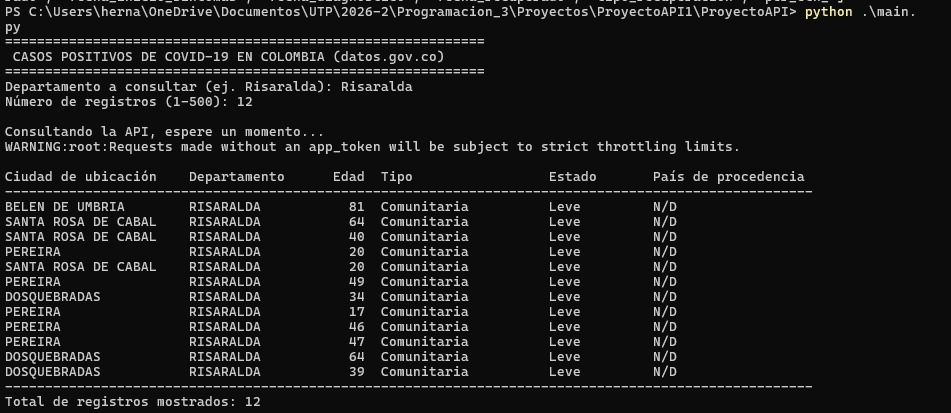
\includegraphics[width=\textwidth]{images/pantallazo1.png}\caption{Consulta 1}\end{figure}}{\textit{(Agregar aquí images/pantallazo1.png)}}

\IfFileExists{images/pantallazo2.png}{\begin{figure}[h!]\centering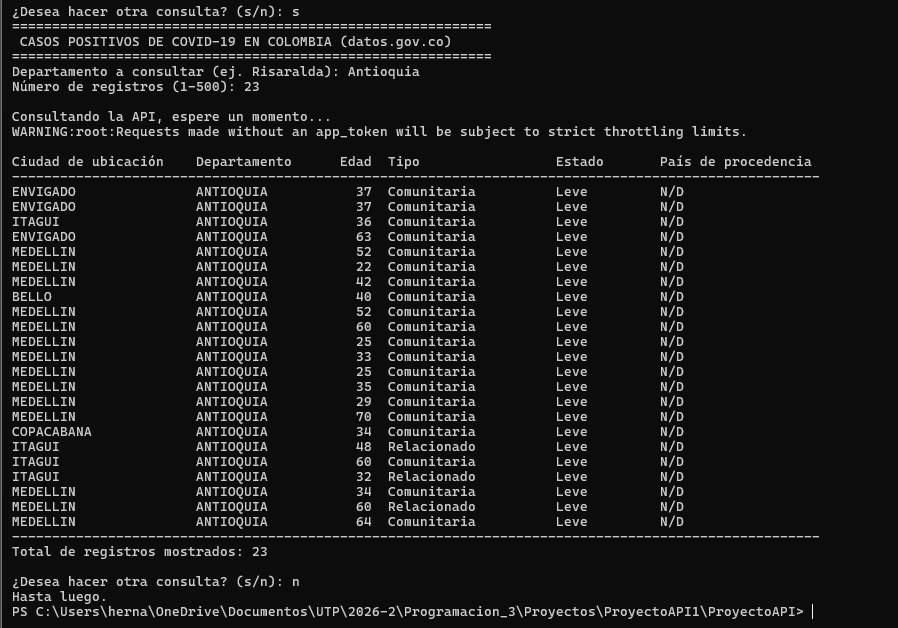
\includegraphics[width=\textwidth]{images/pantallazo2.png}\caption{Consulta 2}\end{figure}}{\textit{(Agregar aquí images/pantallazo2.png)}}

\section{Fundamento teórico: Diagrama de Componentes}

\subsection{¿Qué es un componente?}
Un componente es una parte modular, reemplazable e independiente de un sistema que encapsula su contenido (código y datos) y expone su funcionalidad mediante interfaces bien definidas. Otros componentes lo usan sin necesitar conocer su implementación interna. En este proyecto, \textit{ui}, \textit{api} y \textit{main} son componentes.

\subsection{¿Qué es un Diagrama de Componentes?}
Es un diagrama estructural de UML que muestra cómo se organiza un sistema en componentes y cuáles son las dependencias e interfaces entre ellos.

\subsection{¿Para qué se utiliza?}
Sirve para visualizar la arquitectura de alto nivel, dividir responsabilidades, planificar el trabajo en equipo, facilitar el mantenimiento (se puede cambiar un componente sin afectar a los demás) y comunicar el diseño a otras personas.

\begin{figure}[h!]
    \centering
    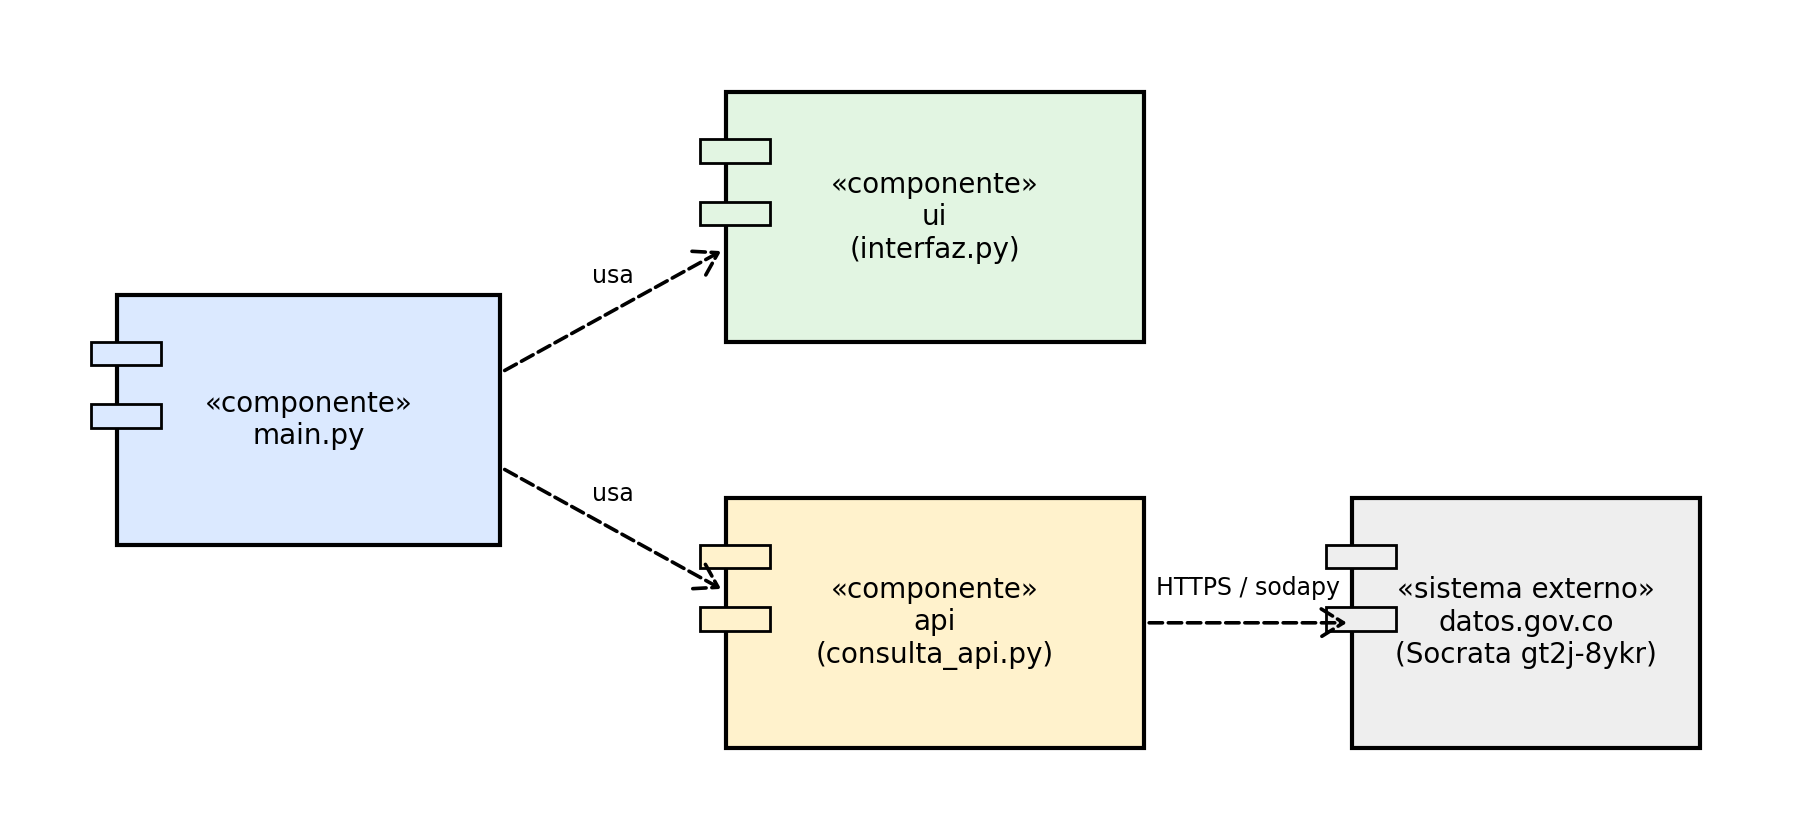
\includegraphics[width=\textwidth]{images/diagrama_componentes.png}
    \caption{Diagrama de componentes del proyecto}
\end{figure}

\textbf{Descripción:} \textit{main} depende de \textit{ui} (pide los datos y muestra el resultado) y de \textit{api} (consulta los casos). El componente \textit{api} se comunica con el sistema externo datos.gov.co a través de la librería \textit{sodapy}. \textit{ui} y \textit{api} no se conocen entre sí, lo que reduce el acoplamiento.

\end{document}